\chapter{The Energy Usage of Template Engine Components}
\label{chapter:comp energy}

Previous chapters have included performance comparisons of software components and the construction and testing of a prototype apparatus to compare the energy use of running software. The results showed that common server applications differ in the energy they use to perform the same task and that there is a wide variety in the performance of software components. Arguably, therefore, both the amount and capability of servers required (which depends to some degree on application performance) and the energy those servers use in operation (which depends on the software they are running) could potentially be reduced by substituting components for ones with better time- and/or energy-efficiency.

This chapter explores the energy usage of software components, in particular the template engines investigated in \autoref{chapter:performance}. A range of experiments are conducted to determine the energy use and its relationship with performance for a range of scenarios. The feasibility of comparing the energy use of software components is considered in \autoref{section:fse}; the experimental approach is improved in \autoref{section:fse2}; and a more realistic scenario is constructed and evaluated in \autoref{section:context energy} to explore the energy and time use of template engines in context.

\section{Performance Tests on Different Platforms}
\label{section:perf dut}

\subsection{Method}

The initial performance experiments in \autoref{chapter:performance} were conducted on a different machine, before the construction of the prototype comparison apparatus. Changing the underlying platform is likely to change the absolute values of the performance measurements, but potentially also the relative performance. To provide context for the energy comparisons in this chapter, the final `Wave 4' performance comparisons were run on the DUT platform of the energy comparison apparatus.

\subsection{Results}
The results are shown in \autoref{results:wave4 dut} and a copy of \autoref{multi:wave4.2-average} for comparison is shown in \autoref{results:wave4 pc}. Note that \autoref{results:wave4 dut} shows the results of a single run without averaging.

\begin{figure}[ht!]
\centering
\includesvg[width=\columnwidth]{Figures/graphs/svg/2024-03-28a.csv.svg}
\caption{\label{results:wave4 dut}Performance Wave 4 Run on the DUT Platform}
\end{figure}

\begin{figure}[ht!]
\centering
\includesvg[width=\columnwidth]{Figures/graphs/svg/2023-12-20avg.csv.svg}
% 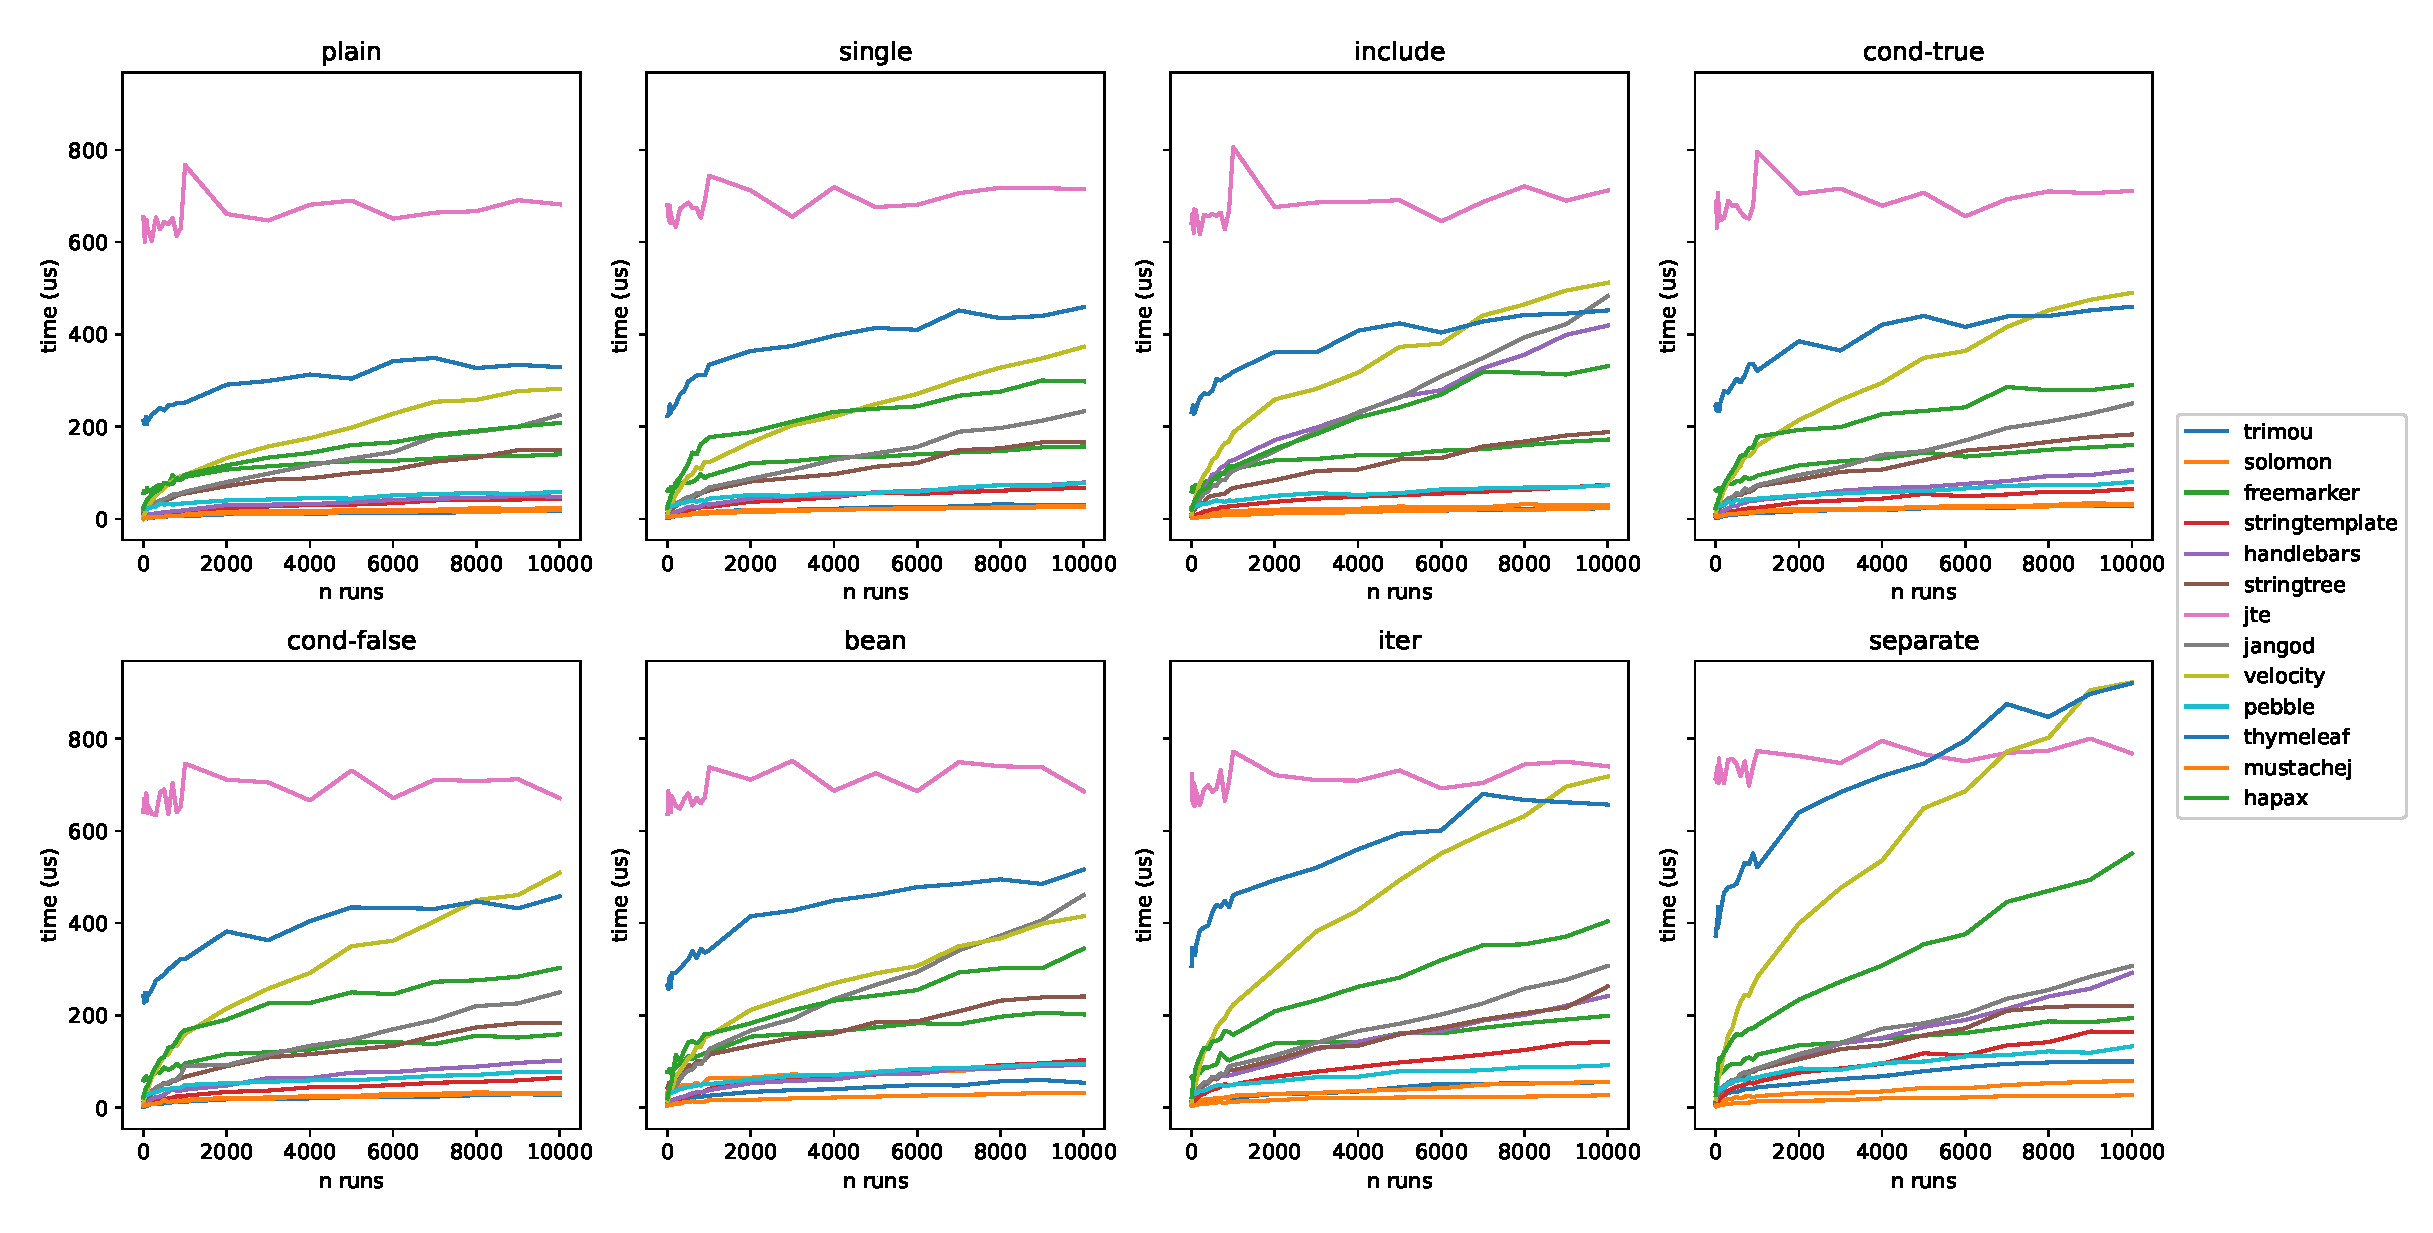
\includegraphics[width=\columnwidth]{Figures/graphs/wave4/2023-12-20avg.eps}
\caption{\label{results:wave4 pc}Performance Wave 4 Run on the Intel PC Platform}
\end{figure}

\subsection{Discussion}

There are several key points to take from the comparison of template engine performance on the two platforms.

All the performance measurements run roughly 10 times the speed on the Intel PC platform compared with the Raspberry Pi-based DUT platform. This, in itself, does not diminish the usefulness of the comparisons, however. neither of these platforms will be identical to current and future web platforms. For this research, the important aspect is the \emph{relative} performance of the different template engines in the different scenarios. The relative performance is indicated by the shapes of the curves and the points at which they cross.

The shapes of the curves in the two sets of measurements are broadly similar. For example, in both cases \emph{JTE} has a relatively high minimum duration and a relatively gentle slope, \emph{Velocity} has a much lower minimum duration but a steeper slope, and \emph{Thymeleaf} is somewhere in between those two. Where the two sets of measurements differ is in the crossing points. Consider the `separate' scenario, for example. On the PC platform, \emph{JTE} becomes a better choice than \emph{Thymeleaf} at around 5000 runs, and a better choice than \emph{Velocity} at around 7000 runs. On the DUT platform, however, \emph{JTE} becomes a better choice than \emph{Thymeleaf} at around 1000 runs, and a better choice than \emph{Velocity} at around 3000 runs. The slope of the graphs indicate that this difference will probably become increasingly important as the number of runs increases beyond 10,000. The effect of this can be seen in the energy comparison timings in \autoref{section:context energy}.  Further research is required to determine which specific differences between the two platforms cause these effects.

A minor, but encouraging, point is that there appears to be considerably less influence of `noise' on the performance measurements on the DUT platform. This is likely to be due in part by the longer time taken for the measurements but the relative simplicity of the operating system installation on the DUT device, with fewer background processes running, may also be a factor.

\section{The Feasibility of Comparing Component Energy Use}
\label{section:fse}

\subsection{Method}
\label{fse methodology}

The apparatus from \autoref{chapter:testrig} had already been used to compare the energy usage of web server software written in Java, so no extra support was needed to run the evaluation scenarios. However, the comparison apparatus had been designed to trigger execution of server code via requests from the \texttt{LOAD} device. To integrate the code from the performance study with this architecture required either changes to the performance study code, or the addition of a server to listen for trigger requests and invoke an appropriate performance study script.

For simplicity, and to minimise any accidental issues due to modification of the performance study code, it was decided to use one of the web servers compared during the evaluation of the apparatus and to invoke the performance study code using the \emph{Common gateway Interface} (CGI) protocol. CGI was designed as a method for invoking local programs from an HTTP request, so seemed a suitable choice for this task. The web server \emph{Lighttpd} had consumed the least energy when serving static pages when evaluated in \autoref{chapter:testrig} so this server was used.

Lighttpd is very configurable and was supplied with an example of the configuration needed to serve CGI requests. All that was required was to modify this configuration slightly: to indicate where to look for scripts to execute when a CGI request is received, and to add a mapping to indicate that shell scripts should be executed by the system shell \verb!/bin/bash!. The configuration changes were tested using a simple `hello world' CGI script.

Once the operation of the server had been confirmed, a CGI script was created which called the \emph{one.sh} script described in \autoref{chapter:performance}. This script evaluates a single template engine by running all the scenarios a specified number of times. For the initial experiments, a count of 1000 times for each scenario was used. As this was just an initial study to determine if any difference in energy consumption could be observed, each template engine was measured just once.

\subsection{Results}
\label{fse results}

The measured net energy use (after subtracting the `baseline' energy use of a quiescent system) for each of the template engines is shown in \autoref{fse:results:net 1000}.

\begin{table}[ht!]
\centering
\begin{tabular}{lccr}
\textbf{Engine} & \textbf{Energy (J)} \\
\hline
freemarker & 11.4936 \\
handlebars & 12.4403 \\
hapax & 10.7424 \\
jangod & 9.33103 \\
jte & 5.13393 \\
mustachej & 7.22679 \\
pebble & 8.48842 \\
solomon & 4.90431 \\
stringtemplate & 6.20053 \\
stringtree & 8.39519 \\
thymeleaf & 15.6721 \\
trimou & 7.98896 \\
velocity & 11.5069 \\
\end{tabular}
\caption{Average net energy use for 1000 sets of scenarios by template engine\label{fse:results:net 1000}}
\end{table}

\subsection{Discussion}
\label{fse discussion}

The results from \autoref{fse:results:net 1000} show a discernible difference in energy usage between the template engines. However, the scale of the difference is considerably less than shown in the performance figures from \autoref{chapter:performance}. Also, the energy use figures from this experiment do not align well with the performance figures. A striking example is \emph{JTE} which exhibited the slowest performance at 1000 repetitions of all the template engines in this cohort (see \autoref{multi:wave4-average}), yet shows the second lowest energy usage in this experiment.

While the energy usage figures from this experiment are interesting, they should not be considered authoritative for several reasons:

\paragraph{Low number of samples}
The typical duration of 1000 repetitions of the suite of template scenarios for these template engines was between 10 and 20 seconds. The experimental test apparatus was configured to sample current and voltage at 1 second intervals which meant that each run only had 10-20 readings from which to derive an average energy figure (see \autoref{fse2:energy single 1000}). The readings varied widely during this period, so it is entirely possible that one or two outliers, either high or low, could noticeably perturb the average.

\begin{figure}[htbp]
  \centering
  % \def\svgwidth{\columnwidth}
  \includesvg[width=\columnwidth]{Figures/graphs/Energy/SingleRun1000.svg}
  \caption{Energy Readings From 1,000 scenarios}
  \label{fse2:energy single 1000}
\end{figure}

\paragraph{System `noise' and other external factors}
The contribution to the energy due to the components in these experiments is small compared to the energy usage of the system as a whole. Background processes and the general functioning of the system add `noise' to the measurements which can, on occasion, overshadow the energy usage of the components. When combined with the low number of samples and the experiment being run only once for each template engine, this also acts to reduce confidence in the comparison.

\paragraph{Unrepresentative scenarios}
The performance experiments in \autoref{chapter:performance} were designed to investigate the differences in behaviour of template engines in specific circumstances. In those experiments it made sense to repeat each specific scenario many times in order to amplify the differences and minimise the influence of external factors. If the intention is to obtain a directly applicable comparison between the energy usage of components when deployed to real applications, then a more representative scenario might be more appropriate.

\paragraph{Platform differences}
The performance experiments in \autoref{chapter:performance} were conducted on an Intel CPU running a 64-bit operating system, while the energy experiments in this section were conducted on the energy measurement apparatus which uses an ARM CPU running a 32-bit operating system. Differences between the performance results for the two different platforms are explored in \autoref{section:perf dut}.

\subsection{Conclusions}
\label{fse conclusions}

The initial conclusions from this experiment were that there was an apparent difference in the energy consumption of the template engine components when tested with the simple scenarios used for the performance comparisons, but further investigation was required. Future experiments would need to include a larger number of cycles within each run and the averaging of several runs to minimise the impact of system noise and other external factors as well as the construction of further, more representative, scenarios.


\section{More Samples and Averaging}
\label{section:fse2}

Following the approach taken in \autoref{section:fs1} and \autoref{section:perf dut}, a further energy comparison experiment was carried out in which each template engine was exercised 10,000 times for each of the performance test scenarios. Both energy use and time taken to process the test scenario were recorded. Each set of 10,000 was repeated three times for each template engine and the results were averaged to reduce the effect of system noise and interference.

\subsection{Results}
\label{fse2 results}

Increasing the number of repetitions of each template scenario served to reduce the variability of the energy readings in most cases. \autoref{fse2:energy single 10000} shows relatively consistent energy use during the measurement, with the addition of noise in a similar manner to the performance graph in \autoref{results:fullsolomon}.

\begin{figure}[htbp]
  \centering
  % \def\svgwidth{\columnwidth}
  \includesvg[width=\columnwidth]{Figures/graphs/Energy/SingleRun10000.svg}
  \caption{Energy Readings From 10,000 runs of \emph{Pebble}}
  \label{fse2:energy single 10000}
\end{figure}

\subsubsection{Energy Use}
\label{fse2 results energy}

\autoref{fse2:energy graph} shows the comparative energy use of the selected template engines with the centre dot representing the average of three runs and the range bars indicating maximum and minimum values. The graph clearly shows a wide variation in energy use between template engines for this scenario.

\begin{figure}[htbp]
  \centering
  % \def\svgwidth{\columnwidth}
  \includesvg[width=\columnwidth]{Figures/graphs/Energy/ComponentEnergy.svg}
  \caption{Averaged Energy Use by Template Engine}
  \label{fse2:energy graph}
\end{figure}

\subsubsection{Time Taken}
\label{fse2 results time}

\autoref{fse2:time graph} shows the time taken for the experiments shown in \autoref{fse2:energy graph}. There is also a wide variation between these figures which has some similarity to the energy usage but also has some important differences. For example, \emph{Hapax} shows as faster than \emph{Jangod}, but achieves that speed at the expense of extra energy usage.

\begin{figure}[htbp]
  \centering
  % \def\svgwidth{\columnwidth}
  \includesvg[width=\columnwidth]{Figures/graphs/Energy/ComponentTime.svg}
  \caption{Averaged Test Duration by Template Engine}
  \label{fse2:time graph}
\end{figure}

\subsubsection{Running Power Consumption}
\label{fse2 results power}

Having recorded both total energy use and time taken for each of the test runs, it became possible to derive the average running power consumption for each of the template engines by dividing the total energy used by the total time taken for each run. These derived values are shown in \autoref{fse2:power graph}.

\begin{figure}[htbp]
  \centering
  % \def\svgwidth{\columnwidth}
  \includesvg[width=\columnwidth]{Figures/graphs/Energy/ComponentPower.svg}
  \caption{Averaged Running Power by Template Engine}
  \label{fse2:power graph}
\end{figure}

\subsection{Discussion}
\label{fse2 discussion}

Unlike the improved performance experiments in \autoref{section:fs2}, the experiments which provided the energy and duration values in this section only represented a single quantity of requests. However, there is a clear variation between the evaluated template engines in both time taken and energy used. 

While the emphasis of this research is on comparing the energy used by different software components, the addition of performance measurements also enables investigation into the running power consumption of the different components and its potential use as an indicator of the relationship between performance and energy use. This relationship between energy use and time taken, as shown in \autoref{fse2:power graph}, is also different for the different template engines. In these results, \emph{Hapax} uses approximately twice the running power of \emph{JTE}. A component which uses less running power is not necessarily a better or worse choice than one which uses more, however. The important values for capacity planning are performance, which can be used to determine the number of machines required to serve a desired number of requests per second, and total energy use, which indicates which components are more or less energy-efficient for the same task.

The disparity in calculated running power, even at a single quantity of repetitions, indicates that performance measurement is a poor analogue for energy use. However, the combination of the different measurements can help decide which components to choose, at least for this kind of scenario on this kind of platform. For example, in this experiment, \emph{Velocity} exhibits both the worst performance and the worst energy use so is unlikely to be a good choice.\emph{JTE}, on the other hand performs consistently well in both performance and energy use. One concern with \emph{JTE} in this scenario is that it completes so quickly that it does not allow enough time for a large number of energy readings.

\subsection{Conclusions}
\label{fse2 conclusions}

This experiment confirms that there is an observable difference in both performance and energy use of different template engine components. Combining the two sets of measurements also shows that the different components have different relationships between performance and energy use. This indicates that, without prior calibration specific to the code being executed, performance measurement is not a reliable way to predict overall energy use.

Results from \autoref{chapter:performance} showed that the different components perform differently under different volumes of requests, but the experiments in this section all used the same volume. It is expected that energy use, time taken, and running power will also vary depending on request volume.  Further experimentation is needed to validate this assumption as well as to determine how well such abstract test scenarios represent real deployments.

\section{Measuring Template Engines in Context}
\label{section:context energy}

\subsection{Introduction and Scope}
\label{cce intro}

The preceding experiments have concentrated on testing the behaviour of specific template engine features. While informative, such scenarios may not be fully representative of the way such template engines are used on the web. To better simulate that kind of usage an example web page was converted to an intermediate template using the \emph{GILT} template language discussed in \autoref{chapter:intermediate}. This intermediate template was then used to generate templates for a selection of template engines. The performance and energy usage of the selected template engines were compared using the apparatus described in \autoref{chapter:testrig}. The results of these comparisons are described in \autoref{cce results}.

\subsection{Methods}

\subsubsection{Selecting A Web Page and Generating Templates}
\label{cce pages}

Web pages on the public internet vary widely. From simple pages holding a single image or a small amount of text to large, sprawling pages containing many distinct sections and structures. For the purposes of this investigation, a page was needed containing representative usage of many of the template features compared in previous sections. Such a web page would need boilerplate text, simple substitutions, template inclusion, iteration through a list, and boolean selection. Method invocation is not supported across the full range of template engines, so that was excluded from this investigation.

The desired set of features are found on many blogs and other similarly-structured sites. The blog page used for the comparison between servers in \autoref{chapter:testrig} only contains the content for a single page with little opportunity for iteration, so it was decided to use the `front page' of a blog which contains multiple tags, archive links, and sections for different blog posts. To avoid potential repeatability issues with relying on an externally-controlled website, a snapshot of the front page of the website and blog associated with this research\footnote{\url{https://greenprogrammer.net/}} was selected.

\subsubsection{Generating Templates}
\label{cce gilt}

The aim of the experiment was to compare the performance and energy use of a range of template engines. In order to do this, templates would be needed in appropriate template languages for each of the engines. The intention was to generate these templates from a single intermediate template coded using the \emph{GILT} intermediate language described in \autoref{chapter:intermediate}. It quickly became clear during the creation of this intermediate template that the only way to test for correctness was to generate a template for one of the candidate template engines and then expand that template using the appropriate template engine. This process was cumbersome, and led to confusion whenever there was an error as to whether the issue was in the intermediate template, the template generation driver for the chosen target template language, or the behaviour of the target template language itself.

To eliminate some of these variables, and allow verification of the correctness of the intermediate template without using it to generate a template in a different template language, a new template engine was created. This template engine, named \emph{gilt-native}, uses the \emph{GILT} intermediate language directly as its template language. This template engine enabled faster development and testing of intermediate templates without the need for third-party template engines and direct comparison of the expanded template with the expected web page. 
% Updated results graphs from \autoref{chapter:fs2} including the new \emph{gilt-native} template engine are shown in \autoref{cce results}.

Once a intermediate template containing uses of all the desired features was complete, the \emph{GILT} template generator was used to generate appropriate templates for each of the template engines.

\subsubsection{Selecting a Test Method}
\label{cce method}

When evaluating the effectiveness of the test rig in \autoref{chapter:testrig}, web pages were served by a selection of servers using both dynamic (Wordpress) and static page data. When comparing performance and energy use of components in \autoref{section:fse} and \autoref{section:fse2}, each test scenario was invoked directly using a script. Both approaches showed clear differences between energy use but in the server-based tests the differences between server implementations had the potential to overshadow the differences between components. In order to directly compare the performance and energy use of the candidate template engines it was decided to run each engine from a script in a similar manner to the component tests.

Scripts from the separate scenario tests were copied and modified to load appropriate context data and invoke each template engine using its \verb!EngineDriver! implementation using its generated template.

\subsubsection{Evaluating the Template Engines}
\label{cce evaluation}

Prior to use on the measurement apparatus, each template engine was invoked with the intended context data and generated template, and the result was compared with the expected web page. This highlighted several problems which needed to be addressed before the performance and energy use of the template engines could be measured and compared.

The most common problems were differences in the handling of `whitespace' such as space, tab, and newline characters. All the template engines in this cohort were designed primarily to generate output formatted using HTML. The rendering of HTML by web browsers is mostly insensitive to the presence or absence of such whitespace, so the template engine developers have not always cared about exactly preserving whitespace when generating web pages. For example, \emph{velocity} failed to preserve a new line following a template inclusion directive (see \autoref{velocity diff}.

\begin{figure}[htbp]
  \centering
  \includegraphics[width=\columnwidth]{Figures/graphs/Page/velocity-diff.png}
  \caption{Difference in generated whitespace}
  \label{velocity diff}
\end{figure}

After examining the output from these template engines, the acceptance criteria for a successful template expansion were widened to allow such minor differences in whitespace.

Other template engines, however, had bigger issues. Even though each of the template engines considered for this phase of the investigation had passed the individual tests in \autoref{chapter:performance}, some failed to generate acceptable output for this more complex scenario. For example, \emph{Solomon}, which had performed flawlessly on the individual scenarios, initially generated a much smaller output file than the other template engines. When the output was examined it was clear that the template inclusion directives had failed. To understand why this was happening, the source code for the \emph{Solomon} template engine was used instead of the provided library, and instrumented to discover the cause of the problem. An issue was discovered in the filenames of the templates to be included. \emph{Solomon} expected the names of included templates to conform to the rules for identifier names in Java: starting with a letter then containing a combination of letters, digits, \verb!_! and \verb!$!. The filenames of the blog post summaries to be included had names beginning with their creation date in the form \verb!2022-10-23! which meant that the filenames were not valid Java identifiers. Once this issue was resolved, by renaming included template file to be valid Java identifiers, \emph{Solomon} generated the correct output. This issue was subsequently raised with the \emph{Solomon} developers, who relaxed this unnecessary restriction in a later release.

Of the remaining template engines, some initially  failed to process the generated template at all.

\emph{JTE}, which had performed well in the tests of individual features, uses an approach which converts a supplied template into Java source code, then compiles that source code and runs it to expand the template. This approach requires additional specialist annotation in templates to enable the correct Java code to be generated. Unlike all the other template engines, which provide access to data values via a shared context visible to all templates, \emph{JTE} requires that context value names and types be declared in a header section at the start of the template. When including one template in another, any context values used in the child template need to be both declared in the child template, and passed as `parameters' in the include directive. During the evaluation of individual template engine features and the development of the \emph{JTE} driver, no child template made use of context values, so this requirement was never discovered. Although the \emph{JTE} driver generated child templates with the correct declarations, it failed to generate the correct `parameters' in the parent template, which in turn meant that \emph{JTE} generated invalid Java code which \emph{JTE} could not compile. To add this feature to the \emph{JTE} driver would require the template generation code to model the complete, transitive, contents of every child template in order to generate a correct parent template. This would require major changes to the architecture of the template generator, so \emph{JTE} was excluded from this phase of the template engine evaluation.

\emph{Stringtemplate} also required included templates to be valid Java identifiers, but once this had been adjusted for \emph{Solomon} the template generation process still produced invalid templates. Further investigation determined that the \emph{Stringtemplate} driver was using incorrect delimiters for some situations. The driver was updated to correct this error, and then \emph{Stringtemplate} correctly processed the generated template.

\emph{Handlebars} crashed when attempting to expand the generated template. Investigation indicated that this was a problem with the specific version of the \emph{Handlebars} library which was being used which made some uses incompatible with recent versions of Java\footnote{\url{https://github.com/swagger-api/swagger-codegen/issues/10966}} \footnote{\url{https://teamtreehouse.com/community/broke-when-adding-blocks}}. Updating the library removed this problem, but revealed further issues. All previous comparisons had been performed with a single version of the \emph{Handlebars} library. Updating to a new version, even if the further issues could be addressed, would raise questions about the comparability of the measurements, so \emph{Handlebars} was also excluded from this phase of the template engine evaluation.

\emph{Mustachej} required some minor changes to the Driver, but otherwise functioned correctly.

\emph{Hapax} does not fully support loops and conditionals, so was excluded from this phase of the template engine evaluation.

\emph{Thymeleaf} employs an HTML-specific syntax which would require altering the intermediate template document in ways which would make it incompatible with the other template engines, so it was also excluded from this phase of the template engine evaluation.

Energy and performance comparisons were therefore performed on the following template engines:
\emph{trimou},
\emph{solomon},
\emph{freemarker},
\emph{stringtemplate},
\emph{stringtree},
\emph{jangod},
\emph{velocity},
\emph{pebble},
\emph{mustachej},
and \emph{gilt-native}.

A script was created to load a specified context and use a single template engine to expand the templates generated from the example website. Each page expansion was run 100,000 times. The overall run of 100,000 expansions was then repeated twice more, and the results averaged, to minimise the impact of external interference.

\subsection{Results}
\label{cce results}

The energy usage of the averaged runs for each template engine are shown in \autoref{cce:energy page 100000} and the time taken by each template engine is shown in \autoref{cce:time page 100000}. These two data sets have been combined to produce running power figures for each template engine, and these results are shown in \autoref{cce:power page 100000}

\begin{figure}[htbp]
  \centering
  % \def\svgwidth{\columnwidth}
  \includesvg[width=\columnwidth]{Figures/graphs/Page/Full-Page-Energy.svg}
  \caption{Energy Usage of 100,000 page expansions}
  \label{cce:energy page 100000}
\end{figure}

\begin{figure}[htbp]
  \centering
  % \def\svgwidth{\columnwidth}
  \includesvg[width=\columnwidth]{Figures/graphs/Page/Full-Page-Time.svg}
  \caption{Time taken for 100,000 page expansions}
  \label{cce:time page 100000}
\end{figure}

\begin{figure}[htbp]
  \centering
  % \def\svgwidth{\columnwidth}
  \includesvg[width=\columnwidth]{Figures/graphs/Page/Full-Page-Power.svg}
  \caption{Average Running Power for 100,000 page expansions}
  \label{cce:power page 100000}
\end{figure}

\subsection{Analysis}
\label{cce analysis}

In \autoref{cce:energy page 100000} there is an observable difference between the energy usage of the different template engines. There is also a clear distinction between two groups of template engines: those which use less than 100J, and the four template engines which consume over 350J for the same scenario. This distinction suggests that there is some key aspect of the design or implementation which differs between the two groups. Investigation of the reason or reasons for this difference is out of scope for this research, but such a large difference could indicate a potentially fruitful area of future research.

The times taken shown in \autoref{cce:time page 100000} largely echo the energy usage results, with the same four template engines taking the longest to process the specified number of template expansions. The relationship between the template engine energy usage and duration is not constant, however. For example, when considering only energy usage, \emph{velocity} is noticeably worse than \emph{stringtemplate}, but for time taken, these positions are reversed. This difference can be clearly seen in \autoref{cce:power page 100000}. \emph{velocity} uses more energy in a shorter time, which shows as a much higher running power consumption.

While the power figures in \autoref{cce:power page 100000} can be useful when comparing components whose energy usage and time taken are roughly similar, they are not indicative of any notion of efficiency. \emph{mustachej}, for example, shows by far the highest running power consumption, but is still among the lowest for total energy consumption and time taken to complete the task.

\section{Discussion}
\label{ce duscussion}

This chapter has explored some different ways of comparing the energy usage of template engine components. Comparing software components is challenging because, unlike full applications, they cannot be executed without other software to configure, initiate, execute, and shut down the components. This external software can potentially influence the time and energy performance of the components. The results in this chapter show that software components do not usually perform identically in different scenarios. 

The experiments have shown clear differences in energy usage between template engine components. The combined individual scenario experiments in \autoref{section:fse2} provide a ranking of template engines by energy usage as shown in the first data column of \autoref{ce rankings}. If considered in isolation, this ranking would seem to provide a way to select the most energy-efficient template engine for a project. However, when the same template engines were compared using the arguably more realistic scenario of generating a complete web page, the rankings were very different as shown in the second data column of \autoref{ce rankings}.

\begin{table}[ht!]
\centering
\begin{tabular}{lrr}
\multirow{2}{*}{Template Engine} 
      & \multicolumn{2}{c}{Energy Efficiency Ranking} \\
& Individual Scenarios & Full Page Generation \\
\hline
freemarker & 8 & 3 \\
gilt-native & - & 8 \\
handlebars & 9 & - \\
hapax & 11 & -\\
jangod & 10 & 6 \\
jte & 1 & - \\
mustachej & 2 & 5 \\
pebble & 6 & 2 \\
solomon & 3 & 1 \\
stringtemplate & 4 & 7 \\
stringtree & 7 & 10 \\
thymeleaf & 12 & - \\
trimou & 5 & 4 \\
velocity & 13 & 9 \\
\end{tabular}
\caption{Comparative energy-efficiency rankings for template engines\label{ce rankings}}
\end{table}

\subsection{Comparisons With the Performance Studies}
\label{ce performance}

The performance studies in \autoref{chapter:performance} could also potentially be used to rank the template engine components based solely on performance. However, these experiments revealed that the various template engines exhibit different performance characteristics based on the overall volume of requests. Any potential rankings based on the performance studies of individual template engine features would only be valid for the specific features being evaluated at that particular request volume. The energy comparisons were performed at fixed request volumes in order to gain a workable number of energy usage samples, but it is expected that energy-efficiency of some template engines would also vary with request volume.

\subsection{The Relationship Between Energy Use and Performance}
\label{ce relationship}

For the components evaluated in this chapter, the relationship between energy usage and time taken was neither constant between template engines nor constant between scenarios. This relationship, formulated as average running power is shown in \autoref{fse2 results power} and \autoref{cce:power page 100000}. In both scenarios the ratio between energy use and time taken, expressed as Joules per second (Watts) ranged from under 0.3 W to around 0.6 W. This variability suggests that models which aim to predict energy usage based on time performance are unlikely to be generally applicable.

\section{Conclusions}
\label{ce conclusions}

The key conclusion drawn from the experiments in this chapter is that different software components can vary widely in both energy usage and performance when performing the same task, and that the relationship between performance and energy usage is not constant across different evaluation scenarios. The implication of this is that models which attempt to predict energy use solely from other measurements such as performance, task complexity, or static analysis of code will not yield generally-applicable results.